
\chapter{Funciones }

\label{floatchap}

\section{Llamadas a funciones}

\label{functionchap} \index{llamada a función} \index{llamada!función}

Usted ya ha visto un ejemplo de una \textbf{llamada a función}:

\begin{verbatim}
>>> type("32")
str
\end{verbatim}

El nombre de la función es \texttt{type}, y despliega el tipo de un
valor o variable. El valor o variable, que se denomina el \textbf{argumento}
de la función, tiene que encerrarse entre paréntesis. Es usual decir
que una función ``toma'' un argumento y ``retorna'' un resultado.
El resultado se denomina el \textbf{valor de retorno}.

\index{argumento} \index{valor de retorno}

En lugar de imprimir el valor de retorno, podemos asignarlo a una
variable:

\begin{verbatim}
>>> b = type("32")
>>> print(b)
<class 'string'>
\end{verbatim}
 

Otro ejemplo es la función \texttt{id} que toma un valor o una variable
y retorna un entero que actúa como un identificador único:

\begin{verbatim}
>>> id(3)
134882108
>>> b = 3
>>> id(b)
134882108
\end{verbatim}
 Cada valor tiene un \texttt{id} que es un número único relacionado
con el lugar en la memoria en el que está almacenado. El \texttt{id}
de una variable es el \texttt{id} del valor al que la variable se
refiere.

\section{Conversión de tipos}

\index{conversión!tipo} \index{conversión}

Python proporciona una colección de funciones que convierten valores
de un tipo a otro. La función \texttt{int} toma cualquier valor y
lo convierte a un entero, si es posible, de lo contrario se queja:

\begin{verbatim}
>>> int("32")
32
>>> int("Hola")
ValueError: invalid literal for int() with base 10: Hola
\end{verbatim}
 \texttt{int} también puede convertir valores de punto flotante a
enteros, pero hay que tener en cuenta que va a eliminar la parte decimal:

\begin{verbatim}
>>> int(3.99999)
3
>>> int(-2.3)
-2
\end{verbatim}
 La función \texttt{float} convierte enteros y cadenas a números de
punto flotante:

\begin{verbatim}
>>> float(32)
32.0
>>> float("3.14159")
3.14159
\end{verbatim}
 Finalmente, la función \texttt{str} convierte al tipo cadena (\texttt{string}):

\begin{verbatim}
>>> str(32)
'32'
>>> str(3.14149)
'3.14149'
\end{verbatim}
 Puede parecer extraño el hecho de que Python distinga el valor entero
\texttt{1} del valor en punto flotante \texttt{1.0}. Pueden representar
el mismo número pero tienen diferentes tipos. La razón para esto es
que su representación interna en la memoria del computador es distinta.

\section{Coerción de tipos}

\index{coerción de tipos} \index{coerción!tipo} \index{división entera}
\index{división!entera}

Podemos sacar provecho de las reglas de conversión automática de tipos,
que se denominan \textbf{coerción de tipos}. Para los operadores matemáticos,
si algún operando es un número \texttt{flotante}, el otro se convierte
automáticamente a \texttt{flotante}:

\begin{verbatim}
>>> minuto = 59
>>> minuto / 60.0
0.983333333333
\end{verbatim}

Así que haciendo el denominador flotante, forzamos a Python a realizar
división en punto flotante.

\section{Funciones matemáticas}

\index{función matemática} \index{función!matemática}

En matemática usted probablemente ha visto funciones como el \texttt{seno}
y el \texttt{logaritmo}, y ha aprendido a evaluar expresiones como
\texttt{sen(pi/2)} y \texttt{log(1/x)}. Primero, se evalúa la expresión
entre paréntesis (el argumento). Por ejemplo, \texttt{pi/2} es aproximadamente
1.571, y \texttt{1/x} es 0.1 (si \texttt{x} tiene el valor 10.0).

Entonces, se evalúa la función, ya sea mirando el resultado en una
tabla o calculando varias operaciones. El \texttt{seno} de 1.571 es
1, y el \texttt{logaritmo} de 0.1 es -1 (asumiendo que \texttt{log}
indica el logaritmo en base 10).

Este proceso puede aplicarse repetidamente para evaluar expresiones
más complicadas como \texttt{log(1/sen(pi/2))}. Primero se evalúa
el argumento de la función más interna, luego la función, y se continúa
así.

Python tiene un módulo matemático que proporciona la mayoría de las
funciones matemáticas. Un módulo es un archivo que contiene una colección
de funciones relacionadas.

\index{módulo}

Antes de que podamos usar funciones de un módulo, tenemos que importarlas:

\begin{verbatim}
>>> import math
\end{verbatim}
 Para llamar a una de las funciones, tenemos que especificar el nombre
del módulo y el nombre de la función, separados por un punto. Este
formato se denomina \textbf{notación punto}.

\index{notación punto}

\begin{verbatim}
>>> decibel = math.log10(17.0)
>>> angulo = 1.5
>>> altura = math.sin(angulo)
\end{verbatim}
 La primera sentencia le asigna a \texttt{decibel} el logaritmo de
17, en base \texttt{10}. También hay una función llamada \texttt{log}
que usa la base logarítmica \texttt{e}.

La tercera sentencia encuentra el seno del valor de la variable \texttt{angulo}.
\texttt{sin} y las otras funciones trigonométricas (\texttt{cos},
\texttt{tan}, etc.) reciben sus argumentos en radianes. Para convertir
de grados a radianes hay que dividir por 360 y multiplicar por \texttt{2{*}pi}.
Por ejemplo, para encontrar el seno de 45 grados, primero calculamos
el ángulo en radianes y luego tomamos el seno:

\begin{verbatim}
>>> grados = 45
>>> angulo = grados * 2 * math.pi / 360.0
>>> math.sin(angulo)
\end{verbatim}
 La constante \texttt{pi} también hace parte del módulo matemático.
Si usted recuerda geometría puede verificar el resultado comparándolo
con la raíz cuadrada de 2 dividida por 2:

\begin{verbatim}
>>> math.sqrt(2) / 2.0
0.707106781187
\end{verbatim}
 

\section{Composición}

\index{composición} \index{función!composición}

Así como las funciones matemáticas, las funciones de Python pueden
componerse, de forma que una expresión sea parte de otra. Por ejemplo,
usted puede usar cualquier expresión como argumento a una función:

\begin{verbatim}
>>> x = math.cos(angulo + math.pi/2)
\end{verbatim}

Esta sentencia toma el valor de \texttt{pi}, lo divide por 2, y suma
este resultado al valor de \texttt{angulo}. Después, la suma se le
pasa como argumento a la función coseno (\texttt{cos}).

También se puede tomar el resultado de una función y pasarlo como
argumento a otra:
\begin{verbatim}
>>> x = math.exp(math.log(10.0))
\end{verbatim}

Esta sentencia halla el logaritmo en base \texttt{e} de 10 y luego
eleva \texttt{e} a dicho resultado. El resultado se asigna a \texttt{x}.

\section{Agregando nuevas funciones}

Hasta aquí solo hemos usado las funciones que vienen con Python, pero
también es posible agregar nuevas funciones. Crear nuevas funciones
para resolver nuestros problemas particulares es una de las capacidades
mas importantes de un lenguaje de programación de propósito general.

En el contexto de la programación, una \textbf{función} es una secuencia
de sentencias que ejecuta una operación deseada y tiene un nombre.
Esta operación se especifica en una \textbf{definición de función}.
Las funciones que hemos usado hasta ahora ya han sido definidas para
nosotros. Esto es bueno, porque nos permite usarlas sin preocuparnos
de los detalles de sus definiciones.

\index{función} \index{función definición} \index{definición!función}

La sintaxis para una definición de función es:

\begin{verbatim}
def NOMBRE( LISTA DE PARAMETROS ):
  SENTENCIAS
\end{verbatim}
 Usted puede inventar los nombres que desee para sus funciones con
tal de que no use una palabra reservada. La lista de parámetros especifica
que información, si es que la hay, se debe proporcionar a fin de usar
la nueva función.

Se puede incluir cualquier número de sentencias dentro de la función,
pero tienen que sangrarse o indentarse a partir de la margen izquierda.
La práctica estándar de Python es usar 4 espacios.

Las primeras funciones que vamos a escribir no tienen parámetros,
así que la sintaxis luce así:

\begin{verbatim}
def nuevaLinea():
  print()
\end{verbatim}
 Esta función se llama \texttt{nuevaLinea}. Los paréntesis vacíos
indican que no tiene parámetros. Contiene solamente una sentencia,
que produce como salida una línea vacía. Eso es lo que ocurre cuando
se usa el comando \texttt{print} sin argumentos.

La sintaxis para llamar la nueva función es la misma que para las
funciones predefinidas en Python:

\begin{verbatim}
print("Primera Linea.")
nuevaLinea()
print("Segunda Linea.")
\end{verbatim}
 La salida para este programa es:
\begin{verbatim}
Primera Linea.

Segunda Linea.
\end{verbatim}
Note el espacio extra entre las dos líneas. ¿Qué pasa si deseamos
más espacio entre las líneas? Podemos llamar la misma función repetidamente:

\begin{verbatim}
print("Primera Linea.")
nuevaLinea()
nuevaLinea()
nuevaLinea()
print("Segunda Linea.")
\end{verbatim}
 

O podemos escribir una nueva función llamada \texttt{tresLineas} que
imprima tres líneas:

\begin{verbatim}
def tresLineas():
  nuevaLinea()
  nuevaLinea()
  nuevaLinea()

print("Primera Linea.")
tresLineas()
print("Segunda Linea.")
\end{verbatim}
 Esta función contiene tres sentencias, y todas están sangradas por
dos espacios. Como la próxima sentencia, \texttt{print("Primera Linea")},
no está sangrada, Python la interpreta afuera de la función.

Hay que enfatizar dos hechos sobre este programa:
\begin{enumerate}
\item Usted puede llamar la misma función repetidamente. De hecho, es una
práctica muy común y útil.
\item Usted puede llamar una función dentro de otra función; en este caso
\texttt{tresLineas} llama a \texttt{nuevaLinea}.
\end{enumerate}
Hasta este punto, puede que no parezca claro porque hay que tomarse
la molestia de crear todas estas funciones. De hecho, hay muchas razones,
y este ejemplo muestra dos:
\begin{itemize}
\item Crear una nueva función le da a usted la oportunidad de nombrar un
grupo de sentencias. Las funciones pueden simplificar un programa
escondiendo un cálculo complejo detrás de un comando único que usa
palabras en lenguaje natural, en lugar de un código arcano.
\item Crear una nueva función puede recortar el tamaño de un programa eliminando
el código repetitivo. Por ejemplo, una forma más corta de imprimir
nueve líneas consecutivas consiste en llamar la función \texttt{tresLineas}
tres veces.
\end{itemize}

\section{Definiciones y uso}

Uniendo los fragmentos de la sección 3.6, el programa completo luce
así:

\begin{verbatim}
def nuevaLinea():
  print()

def tresLineas():
  nuevaLinea()
  nuevaLinea()
  nuevaLinea()

print("Primera Linea.")
tresLineas()
print("Segunda Linea.")
\end{verbatim}
 Este programa contiene dos definiciones de funciones: \texttt{nuevaLinea}
y \texttt{tresLineas}. Las definiciones de funciones se ejecutan como
las otras sentencias, pero su efecto es crear nuevas funciones. Las
sentencias, dentro de la función, no se ejecutan hasta que la función
sea llamada, y la definición no genera salida.

Como usted puede imaginar, se tiene que crear una función antes de
ejecutarla. En otras palabras, la definición de función tiene que
ejecutarse antes de llamarla por primera vez.

\section{Flujo de ejecución}

\index{flujo de ejecución}

Con el objetivo de asegurar que una función se defina antes de su
primer uso usted tiene que saber el orden en el que las sentencias
se ejecutan, lo que denominamos \textbf{flujo de ejecución}.

La ejecución siempre empieza con la primera sentencia del programa.
Las sentencias se ejecutan una a una, desde arriba hacia abajo.

Las definiciones de funciones no alteran el flujo de ejecución del
programa, recuerde que las sentencias que están adentro de las funciones
no se ejecutan hasta que éstas sean llamadas. Aunque no es muy común,
usted puede definir una función adentro de otra. En este caso, la
definición interna no se ejecuta hasta que la otra función se llame.

Las llamadas a función son como un desvío en el flujo de ejecución.
En lugar de continuar con la siguiente sentencia, el flujo salta a
la primera línea de la función llamada, ejecuta todas las sentencias
internas, y regresa para continuar donde estaba previamente.

Esto suena sencillo, hasta que tenemos en cuenta que una función puede
llamar a otra. Mientras se está ejecutando una función, el programa
puede ejecutar las sentencias en otra función. Pero, mientras se está
ejecutando la nueva función, ¡el programa puede tener que ejecutar
\textit{otra} función!.

Afortunadamente, Python lleva la pista de donde está fielmente, así
que cada vez que una función termina, el programa continúa su ejecución
en el punto donde se la llamó. Cuando llega al fin del programa, la
ejecución termina.

¿Cual es la moraleja de esta sórdida historia? Cuando lea un programa,
no lo haga de arriba hacia abajo. En lugar de ésto, siga el flujo
de ejecución.

\section{Parámetros y argumentos}

\label{parameters} \index{parámetro} \index{función!parámetro}
\index{argumento} \index{función!argumento}

Algunas de las funciones primitivas que usted ha usado requieren argumentos,
los valores que controlan el trabajo de la función. Por ejemplo, si
usted quiere encontrar el seno de un número, tiene que indicar cual
es el número. Así que, \texttt{sin} toma un valor numérico como argumento.

Algunas funciones toman más de un argumento. Por ejemplo \texttt{pow}
(potencia) toma dos argumentos, la base y el exponente. Dentro de
una función, los valores que se pasan se asignan a variables llamadas
\textbf{parámetros}.

Aquí hay un ejemplo de una función definida por el programador que
toma un parámetro:

\begin{verbatim}
def imprimaDoble(pedro):
  print(pedro, pedro)
\end{verbatim}
 Esta función toma un argumento y lo asigna a un parámetro llamado
\texttt{pedro}. El valor del parámetro (en este momento no tenemos
idea de lo que será) se imprime dos veces, y después, se imprime una
línea vacía. El nombre \texttt{pedro} se escogió para sugerir que
el nombre que se le asigna a un parámetro queda a su libertad; pero,
en general, usted desea escoger algo mas ilustrativo que \texttt{pedro}.

La función \texttt{imprimaDoble} funciona para cualquier tipo que
pueda imprimirse:

\begin{verbatim}
>>> imprimaDoble('Spam')
Spam Spam
>>> imprimaDoble(5)
5 5
>>> imprimaDoble(3.14159)
3.14159 3.14159
\end{verbatim}
 En el primer llamado de función el argumento es una cadena. En el
segundo es un entero. En el tercero es un flotante (\texttt{float}).

Las mismas reglas de composición que se aplican a las funciones primitivas,
se aplican a las definidas por el programador, así que podemos usar
cualquier clase de expresión como un argumento para \texttt{imprimaDoble}:

\begin{verbatim}
>>> imprimaDoble('Spam'*4)
SpamSpamSpamSpam SpamSpamSpamSpam
>>> imprimaDoble(math.cos(math.pi))
-1.0 -1.0
\end{verbatim}
 Como de costumbre, la expresión se evalúa antes de que la función
se ejecute así que \texttt{imprimaDoble} retorna \texttt{SpamSpamSpamSpam
SpamSpamSpamSpam} en lugar de \texttt{'Spam'{*}4 'Spam'{*}4}.

También podemos usar una variable como argumento:

\begin{verbatim}
>>> m = 'Oh, mundo cruel.'
>>> imprimaDoble(m)
Oh, mundo cruel. Oh, mundo cruel.
\end{verbatim}
 Observe algo muy importante, el nombre de la variable que pasamos
como argumento (\texttt{m}) no tiene nada que ver con el nombre del
parámetro (\texttt{pedro}). No importa como se nombraba el valor originalmente
(en el lugar donde se hace el llamado); en la función \texttt{imprimaDoble},
la seguimos llamando de la misma manera \texttt{pedro}.

\section{Las variables y los parámetros son locales}

\index{variable local} \index{variable!local}

Cuando usted crea una \textbf{variable local} en una función, solamente
existe dentro de ella, y no se puede usar por fuera. Por ejemplo:

\begin{verbatim}
def concatenarDoble(parte1, parte2):
  cat = parte1 + parte2
  imprimaDoble(cat)
\end{verbatim}
 Esta función toma dos argumentos, los concatena, y luego imprime
el resultado dos veces. Podemos llamar a la función con dos cadenas:

\begin{verbatim}
>>> cantar1 = "Pie Jesu domine, "
>>> cantar2 = "Dona eis requiem."
>>> concatenarDoble(cantar1, cantar2)
Pie Jesu domine, Dona eis requiem. Pie Jesu domine, Dona 
eis requiem.
\end{verbatim}

Cuando \texttt{concatenarDoble} termina, la variable \texttt{cat}
se destruye. Si intentáramos imprimirla obtendríamos un error:

\begin{verbatim}
>>> print(cat)
NameError: cat
\end{verbatim}
 Los parámetros también son locales. Por ejemplo, afuera de la función
\texttt{imprimaDoble}, no existe algo como \texttt{pedro}. Si usted
intenta usarlo Python se quejará.

\section{Diagramas de pila}

\label{stackdiagram} \index{diagrama de pila} \index{marco de función}
\index{marco}

Para llevar pista de los lugares en que pueden usarse las variables
es útil dibujar un \textbf{diagrama de pila}. Como los diagramas de
estados, los diagramas de pila muestran el valor de cada variable
y además muestran a que función pertenece cada una.

Cada función se representa por un \textbf{marco}. Un marco es una
caja con el nombre de una función al lado y los parámetros y variables
adentro. El diagrama de pila para el ejemplo anterior luce así:

\adjustpage{-4} \beforefig \centerline{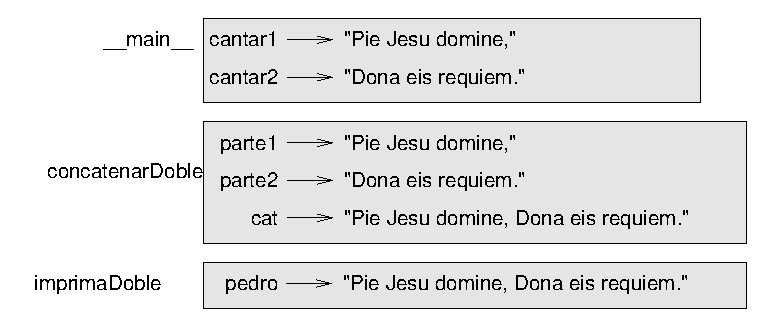
\includegraphics{illustrations/stack}}
\afterfig

El orden de la pila muestra el flujo de ejecución. \texttt{imprimaDoble}
fue llamada por \texttt{concatenarDoble}, y \texttt{concatenarDoble}
fue llamada por \texttt{\_\_main\_\_}, que es un nombre especial para
la función más superior (la principal, que tiene todo programa). Cuando
usted crea una variable afuera de cualquier función, pertenece a \texttt{\_\_main\_\_}.

Cada parámetro se refiere al mismo valor que su argumento correspondiente.
Así que \texttt{parte1} tiene el mismo valor que \texttt{cantar1},
\texttt{parte2} tiene el mismo valor que \texttt{cantar2}, y \texttt{pedro}
tiene el mismo valor que \texttt{cat}.

Si hay un error durante una llamada de función, Python imprime el
nombre de ésta, el nombre de la función que la llamó, y así sucesivamente
hasta llegar a \texttt{\_\_main\_\_}.

Por ejemplo, si intentamos acceder a \texttt{cat} desde \texttt{imprimaDoble},
obtenemos un \texttt{error de nombre (NameError)}:
\begin{verbatim}
Traceback (innermost last):
  File "test.py", line 13, in __main__
    concatenarDoble(cantar1, cantar2)
  File "test.py", line 5, in concatenarDoble
    imprimaDoble(cat)
  File "test.py", line 9, in imprimaDoble
    print(cat)
NameError: cat
\end{verbatim}
Esta lista de funciones se denomina un \textbf{trazado inverso}. Nos
informa en qué archivo de programa ocurrió el error, en qué línea,
y qué funciones se estaban ejecutando en ese momento. También muestra
la línea de código que causó el error.

\index{trazado inverso}

Note la semejanza entre el trazado inverso y el diagrama de pila.
Esto no es una coincidencia.

\section{Funciones con resultados}

Usted ya puede haber notado que algunas de las funciones que estamos
usando, como las matemáticas, entregan resultados. Otras funciones,
como \texttt{nuevaLinea}, ejecutan una acción pero no entregan un
resultado. Esto genera algunas preguntas:
\begin{enumerate}
\item ¿Qué pasa si usted llama a una función y no hace nada con el resultado
(no lo asigna a una variable o no lo usa como parte de una expresión
mas grande)?
\item ¿Qué pasa si usted usa una función sin un resultado como parte de
una expresión, tal como \texttt{nuevaLinea() + 7}?
\item ¿Se pueden escribir funciones que entreguen resultados, o estamos
limitados a funciones tan simples como \texttt{nuevaLinea} y \texttt{imprimaDoble}?
\end{enumerate}
La respuesta a la tercera pregunta es afirmativa y lo lograremos en
el capítulo \ref{funcReturn}.

\section{Glosario}
\begin{description}
\item [{Llamada a función:}] sentencia que ejecuta una función. Consiste
en el nombre de la función seguido por una lista de argumentos encerrados
entre paréntesis.
\item [{Argumento:}] valor que se le da a una función cuando se la está
llamando. Este valor se le asigna al parámetro correspondiente en
la función.
\item [{Valor de retorno:}] es el resultado de una función. Si una llamada
a función se usa como una expresión, el valor de ésta es el valor
de retorno de la función.
\item [{Conversión de tipo:}] sentencia explícita que toma un valor de
un tipo y calcula el valor correspondiente de otro tipo.
\item [{Coerción de tipos:}] conversión de tipo que se hace automáticamente
de acuerdo a las reglas de coerción del lenguaje de programación.
\item [{Módulo:}] archivo que contiene una colección de funciones y clases
relacionadas.
\item [{Notación punto:}] sintaxis para llamar una función que se encuentra
en otro módulo, especificando el nombre módulo seguido por un punto
y el nombre de la función (sin dejar espacios intermedios).
\item [{Función:}] es la secuencia de sentencias que ejecuta alguna operación
útil y que tiene un nombre definido. Las funciones pueden tomar o
no tomar parámetros y pueden entregar o no entregar un resultado.
\item [{Definición de función:}] sentencia que crea una nueva función
especificando su nombre, parámetros y las sentencias que ejecuta.
\item [{Flujo de ejecución:}] orden en el que las sentencias se ejecutan
cuando un programa corre.
\item [{Parámetro:}] nombre usado dentro de una función para referirse
al valor que se pasa como argumento.
\item [{Variable local:}] variable definida dentro de una función. Una
variable local solo puede usarse dentro de su función.
\item [{Diagrama de pila:}] es la representación gráfica de una pila de
funciones, sus variables, y los valores a los que se refieren.
\item [{Marco:}] una caja en un diagrama de pila que representa un llamado
de función. Contiene las variables locales y los parámetros de la
función.
\item [{Trazado inverso:}] lista de las funciones que se estaban ejecutando
y que se imprime cuando ocurre un error en tiempo de ejecución.

\index{llamada a función} \index{valor de retorno} \index{argumento}
\index{coerción} \index{módulo} \index{notación punto} \index{función}
\index{definición de función} \index{flujo de ejecución} \index{parámetro}
\index{variable local} \index{diagrama de pila} \index{marco de función}
\index{marco} \index{trazado inverso}
\end{description}

\section{Ejercicios}
\begin{enumerate}
\item Con un editor de texto cree un guión de Python que se llame pruebame3.py.
Escriba en este archivo una función que se llame \verb+nueveLineas+
que use la función \verb+tresLineas+ para mostrar nueve líneas en
blanco. Enseguida agregue una función que se llame \verb+limpiaPantalla+
que muestre veinticinco líneas en blanco. La última instrucción en
su programa debe ser una llamada a \verb+limpiaPantalla+.
\item Mueva la última instrucción del archivo pruebame3.py al inicio del
programa, de forma tal que la llamada a la función \verb+limpiaPantalla+
esté antes que la definición de función. Ejecute el programa y registre
qué mensaje de error obtiene. ¿Puede establecer una regla sobre las
definiciones de funciones y las llamadas a función que describa la
posición relativa entre ellas en el programa?
\item Escriba una función que imprima la distancia que hay entre dos puntos
ubicados sobre el eje X de un plano cartesiano conociendo sus coordenadas
horizontales.
\item Escriba una función que imprima la distancia que hay entre dos puntos
ubicados sobre el eje Y de un plano cartesiano conociendo sus coordenadas
verticales.
\item Escriba una función que imprima la distancia que hay entre dos puntos
en un plano coordenado, recordando el teorema de Pitágoras.
\item Tome la solución del último ejercicio del capítulo anterior y conviértala
en una función que imprima la nota definitiva de su curso de programación.
\end{enumerate}

